\documentclass[12pt]{article}
\DeclareMathSizes{12}{13}{10}{9}
\usepackage[utf8]{inputenc}
\usepackage[margin=1.5cm]{geometry}
\usepackage{amsmath}
\usepackage{amssymb}
\usepackage{amsthm} % allows example and proof environment to be defined/used
\usepackage{cancel}
\usepackage{graphicx}

\newtheorem*{esempio}{Esempio}

\begin{document}
\section*{Lezione 1}
\subsection*{Rappresentazione dei reali in base b}
Partendo dal seguente fatto (che non dimostriamo, la dimostrazione equivale a costruire i reali $\mathbb{R}$ a partire dai razionali $\mathbb{Q}$): fissata una base $b$ naturale $>$ 1 ogni $x \in \mathbb{R}$ si può scrivere come
\[ \begin{split}
    x & = sign(x)c_mc_{m-1} \dotsc c_1c_0,c_{-1}c_{-2} \dotsc c_{-n} \dotsc \\
    & = sign(x) \biggl( \underbrace{\sum_{j=0}^m c_j b^j}_{\text {parte intera}} + %
    \underbrace{\sum_{j=1}^\infty c_{-j} b^{-j}}_{\text {parte frazionaria}} \biggr) 
\end{split} \]
dove $c_j,c_{-j} \in \{0,1,\dotsc,b-1\}$ sono le cifre della rappresentazione di $x$ in base $b$ e gli indici $j$ e $-j$ corrispondono alle potenze della base, potenze positive per la parte intera e negative per la parte frazionaria.

\begin{esempio} \end{esempio}
\begin{itemize}
    \item $c_j,c_{-j} \in \{0,1,\dotsc,9\}$ base 10
    \item $c_j,c_{-j} \in \{0,1\}$ base 2
    \item $c_j,c_{-j} \in \{0,1,2\}$ base 3
\end{itemize}
Conviene focalizzarsi su:


\begin{itemize}
	\item[$\underline{\textbf{b = 10}}$] la base usuale nelle varie culture umane, corrispondente al fatto che contiamo con 10 dita delle mani, anche se nella storia dell'umanità ci sono state altre scelte:
	\begin{esempio}
	$b = 20$ (Maya) e $b = 60$ (Sumeri)
	\end{esempio}
	\item[$\underline{\textbf{b = 2}}$] la base del calcolatore, corrispondente al fatto che l'unità fondamentale di memoria, il \textit{bit}, può assumere due stati fisici distinti. \\
	Osserviamo che:
	\begin{itemize}
	    \item parte intera $\in \mathbb{N}$
	    \item parte frazionaria $\in [0,1]$
	\end{itemize}
\end{itemize}
La parte frazionaria, in generale, ha $\infty$ cifre e tecnicamente è una serie (somma infinita) a termini non negativi \underline{convergente}.
\begin{esempio}
\underline{base 10}
\[ \begin{split}
    x & = +1278,3405 \dotsc \\
    & = (+1) \cdot (1278 + 0,3405 \dotsc) \\
    & = (+1) \cdot ( \underbrace{1 \cdot 10^3}_{\text {migliaia}} + %
    \underbrace{2 \cdot 10^2}_{\text {centinaia}} + %
    \underbrace{7 \cdot 10^1}_{\text {decine}} + %
    \underbrace{8 \cdot 10^0}_{\text {unità}} + %
    \underbrace{3 \cdot 10^{-1}}_{\text {decimi}} + %
    \underbrace{4 \cdot 10^{-2}}_{\text {centesimi}} + %
    \underbrace{0 \cdot 10^{-3}}_{\text {millesimi}} + %
    \underbrace{5 \cdot 10^{-4}}_{\text {decimill}} + \dotsc) 
\end{split} \]
\end{esempio}
Per far vedere che la serie della parte frazionaria è convergente e quindi rappresenta effettivamente un numero $\in [0,1]$ si usa il criterio di confronto per serie a termini non negativi. \\
Infatti \[ c_{-j}\,b^{-j} \le (b-1)\,b^{-j} \]
perchè \[ 0 \le c_{-j} \le (b-1) \quad \forall \, j \]
quindi \[ \sum_{j=1}^{\infty}c_{-j}b^{-j} \le (b-1)\,\sum_{j=1}^{\infty}b^{-j} \]
e tutto si riduce alla \underline{serie geometrica} di ragione $a = b^{-1} = \frac{1}{b} < 1$ perchè $b > 1$.\\
A questo punto conviene ricordare le proprietà di somma e serie geometrica. 
Chiamiamo \[ S_n = \sum_{j=0}^{n}a^j \quad \text{dove} \quad a \in \mathbb{R} \]
\[ S_n = 1 + a + a^2 + \dotsc + a^n \]
\[ aS_n = a + a^2 + \dotsc + a^n + a^{n+1} \]
quindi \[ aS_n - S_n = (a - 1)\,S_n = a^{n+1} -1 \]
cioè \[ S_n = \frac{a^{n+1} - 1}{a - 1} \quad \text{per} \quad a \ne 1 \]
Ora $a^{n+1}$ diverge per $\lvert a\rvert > 1$ mentre $a^{n+1} \longrightarrow 0 , n \to \infty $ per $\lvert a\rvert < 1$.\\
Allora per $\lvert a\rvert < 1$
\[ \sum_{j=0}^{\infty}a^j = \lim_{n \to \infty} S_n = \frac{1}{1 - a} , \quad \lvert a\rvert < 1 \]
Nel nostro caso $a = b^{-1} < 1$ allora \underline{la serie della parte frazionaria} è maggiorata da una serie geometrica convergente (a meno del fattore $b-1$) e quindi \underline{converge}
\[ \sum_{j=1}^{\infty}c_{-j}b^{-j} \le (b-1)\,\sum_{j=1}^{\infty}b^{-j} < \infty \]
(l'indice parte da $j = 1$ e non da $j = 0$ ma questo ovviamente non cambia niente per la convergenza). \\
Per vedere che la parte frazionaria sta in $[0,1]$, osserviamo che se tutte le cifre dopo la virgola sono uguali alla cifra massima (periodicità sulla cifra massima) la parte frazionaria è 1.

\begin{esempio}
\underline{base 10}
\[ \begin{split}
    (0,\overline{999} \dotsc)_{10} & = \sum_{j=1}^{\infty} 9 \cdot 10^{-j} \\
    & = 9 \cdot \sum_{j=1}^{\infty} 10^{-j} \\
    & = 9 \cdot \biggl( \frac{1}{1 - \frac{1}{10}} - 1 \biggr) \\
    & = 9 \cdot \biggl( \frac{10}{9} - 1 \biggr) \\
    & = 9 \cdot \frac{1}{9} = 1
\end{split} \]
\end{esempio}
\begin{esempio}
\underline{base 2}
\[ \begin{split}
    (0,\overline{111} \dotsc)_{2} & = \sum_{j=1}^{\infty} 1 \cdot 2^{-j} \\
    & = 1 \cdot \sum_{j=1}^{\infty} 2^{-j} \\
    & = \frac{1}{1 - \frac{1}{2}} - 1 \\
    & = 2 - 1 = 1
\end{split} \]
\end{esempio}

Facciamo alcune osservazioni:
\begin{itemize}
    \item i numeri \underline{irrazionali} (as es. $\sqrt{2}$) hanno parte frazionaria infinita (ovvero hanno infinite cifre dopo la virgola) in \underline{qualsiasi base}. Il motivo è che i numeri con parte frazionaria finita in una base sono necessariamente numeri razionali, perchè somma (a meno del segno) della parte intera che è un numero naturale e di una combinazione lineare (i coefficienti sono le cifre delle potenze $b^{-j} = \frac{1}{b^j}$ che sono frazioni);
    \item i numeri razionali possono avere una parte frazionaria finita o infinita a seconda della base
    \begin{esempio} \end{esempio}
    \[ \begin{split}
        \frac{1}{3} & = (0,\overline{333} \dotsc)_{10} \\
        & = (0,100 \dotsc)_{3}
    \end{split} \]
    infatti $\frac{1}{3} = 1 \cdot 3^{-1}$ in base 3. Ma in base 10
    \[ \begin{split}
        (0,\overline{333} \dotsc)_{10} & = \sum_{j=1}^{\infty} 3 \cdot 10^{-j} \\
        & = 3 \cdot \sum_{j=1}^{\infty} 10^{-j} \\
        & = 3 \cdot \frac{1}{9} = \frac{1}{3} \\
        \end{split} 
        \]
\end{itemize}

\subsection*{Errore di troncamento}
A questo punto possiamo affrontare la prima questione fondamentale: siccome nel calcolatore per rappresentare un numero reale (tipicamente in base 2) avremo a disposizione una quantità finita di cifre, che \underline{\textbf{ERRORE}} si fa approssimando un numero reale "tagliando" la parte frazionaria ad $n$ cifre? Cioè utilizzando quello che si chiama il \underline{\textbf{TRONCAMENTO}} ad $n$ cifre della parte frazionaria? \\
Qui cominciano ad entrare in gioco due concetti chiave e pervasivi del calcolo numerico: il concetto di \underline{approssimazione} e il concetto di \underline{errore}. \\
Gli oggetti che si usano (numeri, funzioni, vettori, $\dotsc$) non sono praticamente mai esatti ma sono \underline{approssimati} a meno di un certo errore. La cosa importante è stimare questi errori e studiare il loro effetto nei calcoli (propagazione degli errori). \\
Concentriamoci ora sull'errore di troncamento ad $n$ cifre.\\
Dato \[ x = sign(x) \biggl( \sum_{j=0}^m c_j b^j + \sum_{j=1}^\infty c_{-j} b^{-j} \biggr) \]
definiamo \[ \Tilde{x}_n = sign(x) \biggl( \sum_{j=0}^m c_j b^j + \sum_{j=1}^n c_{-j} b^{-j} \biggr) \]
cioè stesso segno, stessa parte intera e parte frazionaria "tagliata" ad $n$ cifre. \\
In generale definiamo errore su una quantità $a \in \mathbb{R}$ approssimata da $\Tilde{a} \in \mathbb{R}$ (scriveremo $\Tilde{a} \approx a$ per indicare che $\Tilde{a}$ approssima $a$) la quantità \[ \text{ERRORE}\,= \lvert \, a - \Tilde{a} \,\rvert = \lvert \, \Tilde{a} - a \,\rvert \]
quindi ora cerchiamo di stimare $\lvert \, x - \Tilde{x}_n \,\rvert$. \\
È chiaro che \[ \lvert \, x - \Tilde{x}_n \,\rvert = \sum_{j=n+1}^\infty c_{-j} b^{-j} \]
cioè l'errore di troncamento ad $n$ cifre non è altro che il \underline{resto} della serie che definisce la parte frazionaria. Andiamo a calcolare questo resto ragionando come prima, visto che $c_{-j} \le b - 1$ otteniamo
\[ \sum_{j=n+1}^{\infty} c_{-j}b^{-j} \le (b-1)\sum_{j=n+1}^{\infty} b^{-j} \]
quindi basta calcolare il resto della serie geometrica per avere una stima. \\
Ora
\[ \begin{split}
    \sum_{j=n+1}^{\infty} b^{-j} & = \sum_{j=0}^{\infty} b^{-j} - \sum_{j=0}^{n} b^{-j} \\
    & = \frac{1}{1 - b^{-1}} - \frac{1 - b^{-(n+1)}}{1 - b^{-1}} \\
    & = \frac{b^{-(n+1)}}{1 - b^{-1}} \\
    & = \frac{b^{-(n+1)}}{1 - b^{-1}} \\
    & = \frac{b\,b^{-(n+1)}}{b - 1} \\
    & = \frac{b^{-n}}{b - 1}
\end{split} \]
da cui
\[ \begin{split}
    \lvert \, x - \Tilde{x}_n \,\rvert & = \sum_{j=n+1}^\infty c_{-j} b^{-j} \\
    & \le (b-1)\sum_{j=n+1}^{\infty} b^{-j} \\
    & = (b-1) \cdot \frac{b^{-n}}{b - 1} = b^{-n}
\end{split}\]
Cioè abbiamo ricavato una stima dell'errore di troncamento ad $n$ cifre (in una base generica $b$) \[ \lvert \, x - \Tilde{x}_n \,\rvert \le b^{-n} \]
\textbf{ATTENZIONE:} non abbiamo "calcolato" l'errore, ma lo abbiamo \underline{stimato}. \\
Questa è una situazione tipica del calcolo numerico: gli errori di solito non sono noti ma si riesce a ricavarne una stima, talvolta rigorosa (disuguaglianza come in questo caso), spesso meno rigorosa ma in grado di dare almeno un ordine di grandezza all'errore. \\
Il fatto di avere una stima (da sopra) permette comunque di \underline{controllare} l'errore. \\
In questo caso la domanda è: quante cifre devo prendere dopo la virgola (cioè, della parte frazionaria) per garantire che l'errore non superi una fissata tolleranza $\varepsilon > 0$? \\
Basterà che la stima dell'errore non superi $\varepsilon$, infatti
\[ \lvert \, x - \Tilde{x}_n \,\rvert \le b^{-n} \le \varepsilon\]
Se la disuguaglianza $b^{-n} \le \varepsilon$ è soddisfatta, anche l'errore sarà $\le \varepsilon$ (la tolleranza ovviamente dipende dal problema applicativo in cui si utilizza l'approssimazione della quantità cercata).\\
Risolvendo $b^{-n} \le \varepsilon$ come $e^{-n \log b} \le e^{\log \varepsilon}$ si ricava $-n \log b \le \log \varepsilon$ cioè $n \ge - \frac{\log \varepsilon}{\log b}$ quindi perchè l'errore di troncamento sia sicuramente sotto la tolleranza basta prendere il più piccolo numero intero $\ge - \frac{\log \varepsilon}{\log b}$.

\subsection*{Errore di arrotondamento}
In realtà la tecnica di approssimazione più usata non è il troncamento, bensì l'\underline{\textbf{ARROTONDAMENTO}}. Ricordiamo questa tecnica che tutti già conosciamo dalle scuole. \\
Si approssima 
\[ \begin{split}
    x & = sign(x)\biggl( \sum_{j=0}^m c_j b^j + \sum_{j=1}^\infty c_{-j} b^{-j} \biggr) \\
    & = sign(x) \biggl( \sum_{j=0}^m c_j b^j + 0,c_{-1}c_{-2} \dotsc c_{-n} \dotsc \biggr) 
\end{split} \]
con \[ \Tilde{x}_n^{arr} = sign(x) \biggl( \sum_{j=0}^m c_j b^j + 0,c_{-1}c_{-2} \dotsc \Tilde{c}_{-n} \biggr) \]
dove \[\Tilde{c}_{-n} = 
\begin{cases}
    c_{-n} & \text{se $c_{-(n+1)} < \frac{b}{2} \quad \longrightarrow DIFETTO$} \\
    c_{-n}+1 & \text{se $c_{-(n+1)} \ge \frac{b}{2} \quad \longrightarrow ECCESSO$}
\end{cases}
\]
cioè si tiene l'$n$-esima cifra dopo la virgola se la $(n+1)$-esima è minore di metà della base (0, 1, 2, 3, 4 in base 10) che si chiama arrotondamento \underline{per difetto}, invece si aggiunge 1 all'$n$-esima cifra se la $(n+1)$-esima è maggiore o uguale a metà della base (5, 6, 7, 8, 9 in base 10) che si chiama arrotondamento \underline{per eccesso}.\\
In questa discussione ci limitiamo alle basi pari che sono quelle più usate nel calcolo (tipicamente la base 10 e la base 2). \\
Nel caso di basi pari si può dimostrare che
\[ \lvert \, x - \Tilde{x}_n^{arr} \,\rvert \le \frac{b^{-n}}{2}\]
cioè il \underline{massimo} errore di \underline{arrotondamento} ad $n$ cifre dopo la virgola è \underline{metà} del \underline{massimo} errore di \underline{troncamento} ad $n$ cifre (questo non significa che l'errore di arrotondamento sia sempre metà dell'errore di troncamento, come si vede nell'esempio grafico qui sotto).\\
La dimostrazione che si può fare usando la rappresentazione come serie della parte frazionaria è abbastanza difficile, ci accontenteremo di avere una spiegazione grafica con un esempio numerico.
\begin{esempio} \end{esempio}
Consideriamo $b=10$ e $n=2$ e prendiamo i seguenti numeri sull'asse reale \newline
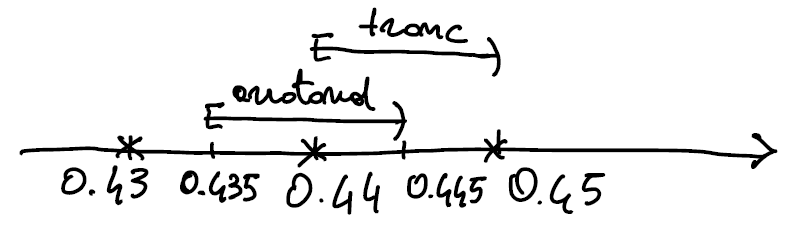
\includegraphics[width=\linewidth]{img1}

Vediamo quali numeri sono approssimati da 0,44 per troncamento e per arrotondamento a 2 cifre (notiamo che qui abbiamo numeri del tipo $0,\dotsc$ che quindi coincidono con la propria parte frazionaria).\\
Per \underline{troncamento} 0,44 approssima tutti i numeri dell'intervallo $[0,44 , 0,45)$ che sono del tipo $0,44\dotsc$ (escluso $0,44\overline{999}\dotsc = 0,45$).\\
Invece per \underline{arrotondamento} approssima tutti i numeri dell'intervallo $[0,435 , 0,445)$ \\ 
Infatti approssima per \underline{difetto} tutti i numeri del tipo \[ 0,440\dotsc \] \[ 0,441\dotsc \] \[ 0,442\dotsc \] \[ 0,443\dotsc \] \[ 0,444\dotsc \]
Mentre approssima per \underline{eccesso} tutti i numeri del tipo \[ 0,435\dotsc \] \[ 0,436\dotsc \] \[ 0,437\dotsc \] \[ 0,438\dotsc \] \[ 0,439\dotsc \]
In pratica l'intervallo di troncamento è un intorno destro di $0,44$ di ampiezza $10^{-2}$, mentre l'intervallo di arrotondamento è un intorno simmetrico di raggio $\frac{10^{-2}}{2}$ e ampiezza $10^{-2}$.\\
Risulta evidente dal punto di vista grafico che l'estremo superiore degli errori di troncamento sia $= 10^{-2}$ (entrambi sono intervalli semi aperti a destra) mentre il massimo degli errori di arrotondamento è $\frac{10^{-2}}{2}$ e si ottiene per $x = 0,435$.
\end{document}